\chapter{Especificação de Requisitos do Sistema}
    Escolhemos especificar os requisitos de sistema do nosso projeto seguindo o modelo de referência ODP, pois ele apresenta uma forma de simplificar a descrição de sistemas complexos por meio dos seus Pontos de Vista.\cite{odppart1} Sabíamos também que gostaríamos se seguir alguns princípios de projeto, descritos na Tabela \ref{principios_de_projeto}. Esses princípios foram resultado de conversas com engenheiros de software e interessados no projeto, e nos ajudaram a guiar durante a definição dos requisitos de sistema.
    \begin{table}
        \centering
        \caption{Princípios de Projeto}
        \label{principios_de_projeto}
        \resizebox{\textwidth}{!}{%
        \begin{tabular}{|l|p{10cm}|}
            \hline
            Princípio de Projeto                 & Descrição \\ \hline
            Ambientes de curta duração           & O desenvolvedor deve ser capaz de criar e deletar ambientes com rapidez e facilidade                                 \\ \hline
            Visualização de fluxos complexos     & O desenvolvedor deve ser capaz de visualizar o resultado de suas requisições HTTP e mensagens Kafka                  \\ \hline
            Ambiente parecido com o local        & O desenvolvedor deve ter uma experiência de desenvolvimento similar com o ambiente de sua máquina                    \\ \hline
            Esconde complexidade de configuração & O desenvolvedor não deve precisar conhecer a configuração dos serviços que ele precisa disponíveis no ambiente dele. \\ \hline
        \end{tabular}
        }
        \legend{Fonte: os autores}
    \end{table}
	\section{Ponto de Vista da Empresa}
	    As empresas que podem se beneficiar do nosso projeto devem ter alguma semelhança com o processo de negócio de desenvolvimento e entrega de novas funcionalidades, descritos respectivamente nas Figuras \ref{fig:build-ci} e \ref{fig:automated-deploy}. O primeiro processo descreve como uma alteração de código por um desenvolvedor gera novas imagens Docker, que são guardadas em um catálogo chamado \textit{Docker Registry}. Exemplos de \textit{Docker Registry} são o DockerHub e o Quay.io. Já o segundo processo, descreve como uma imagem desses catálogo é implantada de forma automatizada pelo Servidor de Entrega Contínua.
	    \begin{figure}[htb]
    	    \centering
    	    \caption{Processo de Entrega Contínua - Construção da imagem Docker}
    	    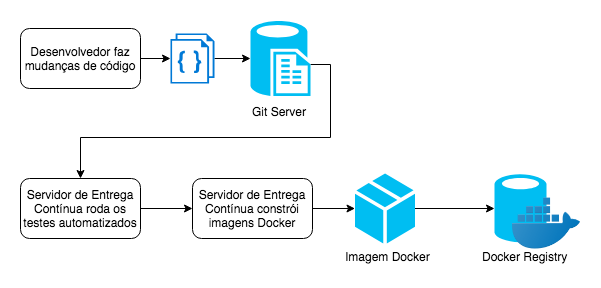
\includegraphics[scale=0.7]{pictures/especificacao-de-requisitos/build-ci.png}
    	    \legend{Fonte: os autores}
    	    \label{fig:build-ci}
	    \end{figure}
	    \begin{figure}[htb]
    	    \centering
    	    \caption{Processo de Entrega Contínua - Implantação automatizada}
    	    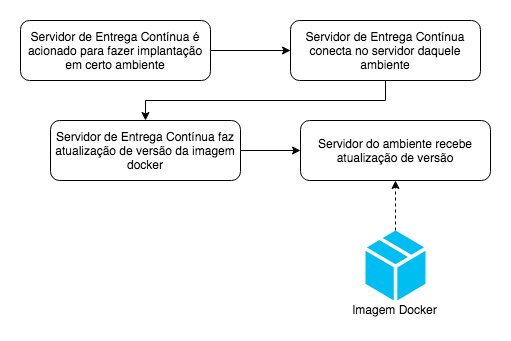
\includegraphics[scale=0.7]{pictures/especificacao-de-requisitos/automated-deploy.png}
    	    \legend{Fonte: os autores}
    	    \label{fig:automated-deploy}
	    \end{figure}
	\section{Ponto de Vista da Informação}
	    O objetivo dessa seção é apresentar a organização das informações por todos os componentes do sistema. A Figura \ref{fig:info-contexts} representa os três principais contextos onde as informações são modeladas, e como é o fluxo de informações. 
	    \begin{figure}[htb]
    	    \centering
    	    \caption{Contextos de informação e seu fluxo}
    	    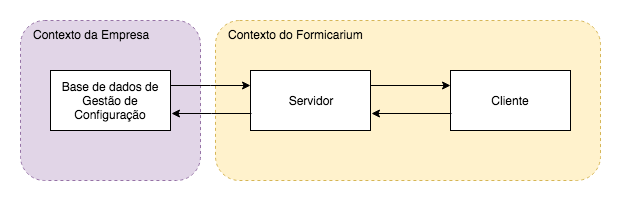
\includegraphics[scale=0.67]{pictures/especificacao-de-requisitos/information-contexts.png}
    	    \legend{Fonte: os autores}
    	    \label{fig:info-contexts}
	    \end{figure}
	    \subsection{Contexto da Empresa}
	        O contexto da empresa refere-se a uma base de dados pré-existente capaz de fornecer as configurações de uma aplicação dado o ambiente: teste, homologação e produção, tradicionalmente. Assim, a modelagem dessa base de dados pode ser arbitrária em relação ao sistema do Formicarium.
	    \subsection{Contexto do Formicarium}
	        \subsubsection{Servidor}
	        A Figura \ref{fig:info-server} representa a modelagem da configuração necessária para rodarmos uma aplicação. Note que uma aplicação pode possuir múltiplas interfaces e pode constituir por múltiplos contêineres. Isso permite maior flexibilidade na implantação e modelagem de aplicações.
	        \begin{figure}[htb]
        	    \centering
        	    \caption{Modelagem das Informações no Servidor}
        	    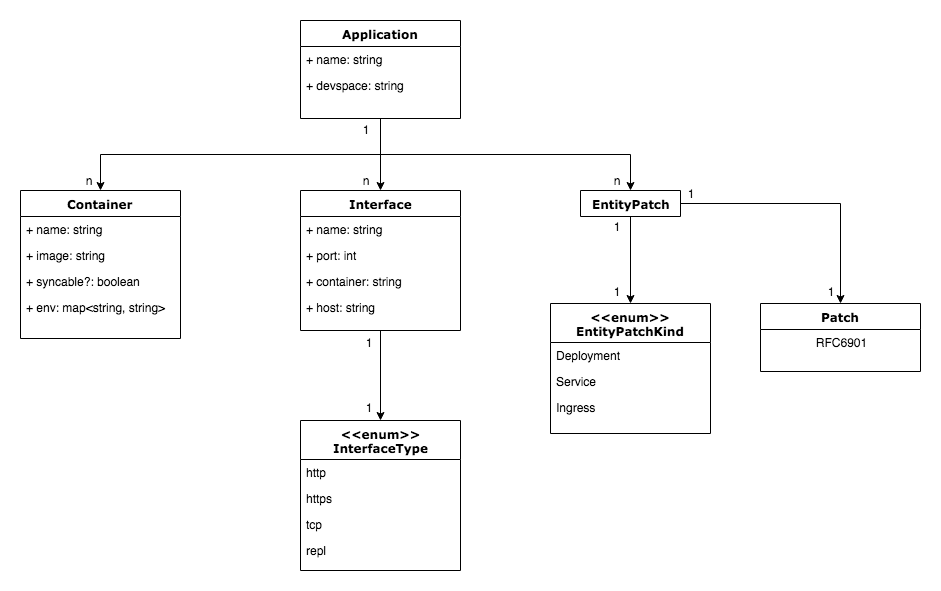
\includegraphics[scale=0.40]{pictures/especificacao-de-requisitos/info-server.png}
        	    \legend{Fonte: os autores}
        	    \label{fig:info-server}
	        \end{figure}
	        \subsubsection{Cliente}
	            
	\section{Ponto de Vista da Computação}
	    O Ponto de Vista da computação está diretamente ligado a distribuição. Não diz respeito aos mecanismos de interação, mas decompõe o sistem em objetos capazes de realizar funções e interagir por interfaces bem definidas \cite{odppart1}.
	    \subsection{Arquitetura de Referência}
	        A arquitetura deste projeto compartilha conceitos e mecanismos com arquiteturas de Plataformas como Serviço (\textit{Platform as a Service}), em particular a arquitetura do Heroku.
	        
	        O Heroku se descreve da seguinte forma: "Heroku é uma plataforma de nuvem baseada em um sistema de contêineres gerenciado, com integração a serviços de dados e um poderoso ecossistema, para implantação e execução de aplicações modernas. O \textit{Heroku Developer Experience} é uma abordagem centrada na aplicação para entrega de software, integrada com as mais populares ferramentas e fluxos de trabalhos atuais." (\citeauthor{herokuplatform}, \citeyear{herokuplatform}).
	        
	\section{Ponto de Vista da Engenharia}
	\section{Ponto de Vista da Tecnologia}
